\documentclass[preview]{standalone}
\usepackage[siunitx, american]{circuitikz}
\usetikzlibrary{positioning, arrows.meta}

\tikzset{
	% 1. Válvula Forrester con máscara de fondo (=== X ===)
	pics/sdvalve/.style={
		code={
			\fill[white] (-0.3, -0.25) rectangle (0.3, 0.25);
			\draw[thick, fill=white] (-0.25, 0.2) -- (0,0) -- (-0.25, -0.2) -- cycle;
			\draw[thick, fill=white] (0.25, 0.2) -- (0,0) -- (0.25, -0.2) -- cycle;
			\draw[thick] (-0.25, 0.2) -- (-0.25, -0.2);
			\draw[thick] (0.25, 0.2) -- (0.25, -0.2);
		}
	},
	% 2. Nube clásica de Forrester
	pics/sdcloud/.style={
		code={
			\draw[xscale=0.10, yscale=0.18,semithick, fill=blue!0] 
			(-3, 0) .. controls (-4, 1.2) and (-1.8, 1.2) .. (-1.4, 0.8)		
			.. controls (-0.9, 1.8) and (0.9, 1.8) .. (1.4, 0.8)		
			.. controls (1.8, 1.2) and (4, 1.2) .. (3, 0);
			\draw[xscale=0.10, yscale=0.18, semithick, fill=blue!0] 
			(-3, 0) .. controls (-4, -1.2) and (-1.8, -1.2) .. (-1.4, -0.8)		
			.. controls (-0.9, -1.8) and (0.9, -1.8) .. (1.4, -0.8)		
			.. controls (1.8, -1.2) and (4, -1.2) .. (3, 0);			
		}
	},
	% 3. Icono de Parámetro nativo de AnyLogic
	pics/alparam/.style={
		code={
			\draw[thick, fill=white] (0,0) circle (0.19);
			\draw[fill] (-0.01, 0.02) -- (-0.12, 0.25) -- (-0.23, 0.15) -- cycle;
		}
	},	
	pics/alparal/.style={
		code={
			\draw[thick, fill=white] (0,0) circle (0.19);
			\draw[fill] (0.01, 0.02) -- (0.12, 0.25) -- (0.23, 0.15) -- cycle;
		}
	}	
}

\begin{document}
	
	\resizebox{\textwidth}{!}{%
		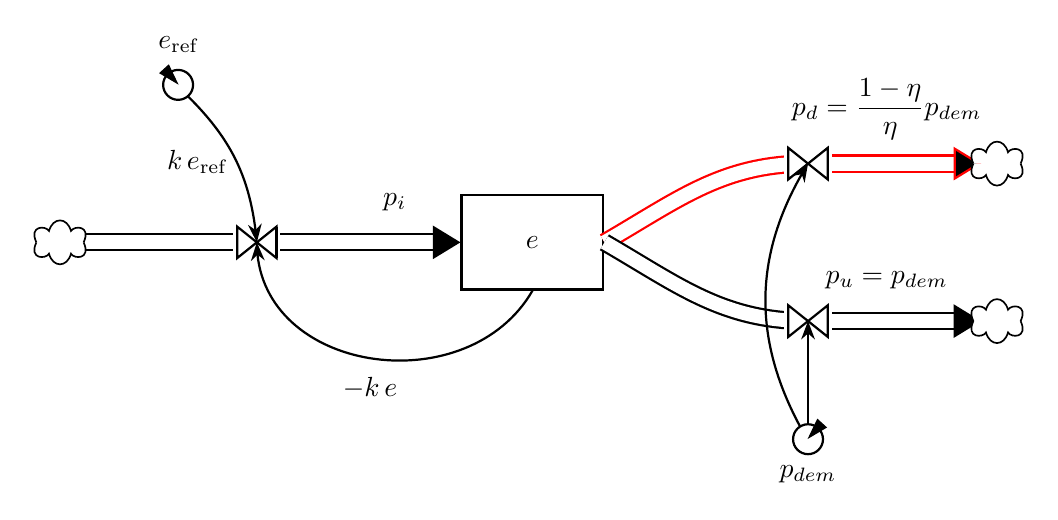
\begin{tikzpicture}[
			stock/.style={rectangle, draw=black, thick, minimum width=1.8cm, minimum height=1.2cm, fill=white, align=center},
			flow/.style={
				draw=black, 
				thick, 
				double, 
				double distance=5pt, 
				fill=white
			},
			% SOLUCIÓN 1: El estilo corregido con fill=black debe ir aquí para evitar conflictos
			flow_arrow/.style={
				flow,
				-{Triangle[length=10pt, width=12pt, fill=black]} 
			},
			sdarrow/.style={-Stealth, thick, >=Stealth}
			]
			
			% =========================================================================
			% CAPA 0: COORDENADAS DE REFERENCIA
			% =========================================================================
			\coordinate (e1_pos) at (0,4);      
			\coordinate (c_in1) at (-6, 4);     
			\coordinate (v_in1) at (-3.5, 4);   	
			\coordinate (v_out1) at (3.5, 5);   
			\coordinate (c_out1) at (6, 5);     
			\coordinate (v_hack) at (3.5, 3);   
			\coordinate (c_hack) at (6, 3);     
			\coordinate (eref1) at (-4.5, 6.0);
			\coordinate (pd1) at (3.5, 6.5);
			\coordinate (ph) at (3.5, 1.5);     
			
			% --- PASO PREVIO: Declaramos el Stock antes para poder usar sus bordes ---
			\node[stock] (e1) at (e1_pos) {$e$};
			
			% =========================================================================
			% CAPA 1: DIBUJO DE FLUJOS 
			% =========================================================================
			% Entrada pi1
			\draw[flow] (c_in1) -- (v_in1);
			% SOLUCIÓN 2: Apuntamos al borde del stock (e1.west) para que la punta no quede oculta debajo
			\draw[flow_arrow] (v_in1) -- (e1.west);
			\node[above=8pt, scale=1.0] at (-1.75, 4) {$p_{i}$};
			
			% Salida pd 
			\draw[flow,draw=red] (e1.east) to[out=30, in=180] (v_out1);
			% SOLUCIÓN 3: Se ajusta la punta final un poco antes para que no invada el centro de la nube
			\draw[flow_arrow,draw=red] (v_out1) -- (5.7, 5); 
			
			% Salida p_dis 
			\draw[flow] (e1.east) to[out=-30, in=180] (v_hack);
			\draw[flow_arrow] (v_hack) -- (5.7, 3); 
			
			\node[above=8pt, scale=1.0] at (4.5, 4.9) {$p_{d} = \displaystyle \frac{1-\eta}{\eta}p_{dem}$};		 
			\node[above=8pt, scale=1.0] at (4.5, 3) {$p_{u} = p_{dem}$};	
			
			% =========================================================================
			% CAPA 2: COMPONENTES OPACOS 
			% =========================================================================
			% --- VÁLVULAS Y NUBES ---
			\pic at (v_in1) {sdvalve};
			\pic at (v_out1) {sdvalve};
			\pic at (v_hack) {sdvalve};
			\pic at (c_in1) {sdcloud};  
			\pic [xshift=-1mm] at (c_out1) {sdcloud}; 
			\pic [xshift=-1mm] at (c_hack) {sdcloud}; 	
			% --- PARÁMETROS ESTILO ANYLOGIC ---
			\pic at (eref1) {alparam};
			\node[above=8pt] at (eref1) {$e_{\text{ref}}$};
			\pic at (ph) {alparal};
			\node[below=6pt] at (ph) { $p_{dem}$};
			
			% =========================================================================
			% CAPA 3: LAZOS DE INFORMACIÓN 
			% =========================================================================
			\draw[sdarrow] (eref1)+(.12,-.14) to [bend left=20] node[left] {$k\,e_{\text{ref}}$}  (v_in1);
			\draw[sdarrow] (e1.south) to[out=-120, in=-90, looseness=1.2] node[midway, below=3pt] {$-k\,e$} (v_in1);
			\draw[sdarrow] (ph)+(0,.2) to  (v_hack);
			\draw[sdarrow] (ph)+(-0.1,0.16) to [bend left=30] (v_out1);
		\end{tikzpicture}
	}
	
\end{document}
